%%%%%%%%%%%%%%%%%%%%%%%%%%%%%%%%%%%%%%%%%%%%%%%%%%%%%%%%%%%%%%%%%%%%%%%
%% Document: Thesis for PhD at UC Riverside                          %%
%% Description: A comparative analysis of environment sensing in EDF %%
%% Author: Steven Ahrendt                                            %%
%%%%%%%%%%%%%%%%%%%%%%%%%%%%%%%%%%%%%%%%%%%%%%%%%%%%%%%%%%%%%%%%%%%%%%%
% RHODOPSIN FIGURES %
%%%%%%%%%%%%%%%%%%%%%

% Presence/absence heatmap for photosensory proteins and accessory components
\begin{figure}[hb]
  \centering
  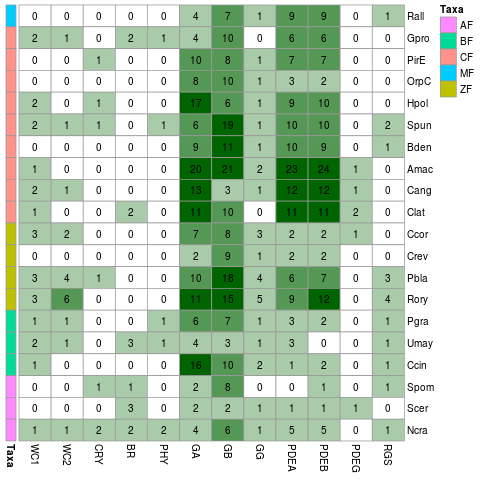
\includegraphics[width=4in]{./Chapter_RhodAux/img/photosenseHeatmap.png}
  \caption[Photosensory survey]{Photosensory protein distribution and G protein signalling pathway component distribution}
  \label{fig:ChRhodA_photosenseSurvey}
\end{figure}

% Galpha msa
\begin{figure}[hb]
  \centering
  \begin{texshade}{./Chapter_RhodAux/dat/FungalGA_PM.fasta_aln}
    \threshold[80]{50}
    \setdomain{1}{1..15,340..355}
    \showruler{1}{top}
    \feature{top}{1}{MGXXXS}{brace[Red]}{Myristoylation [Red]}
    \feature{top}{1}{351..355}{brace[Blue]}{Pertussis [Blue]}
    \hidenumbering
  \end{texshade}
  \caption[Galpha MSA]{Multiple sequence aligment of N-termini and C-termini. G$\alpha$ proteins identified in fungi which posessed both N-terminal myristoylation (MGXXXS) and C-terminal pertussis (C[GAVLIP]{2}X) motifs were aligned using T-coffee.}
  \label{fig:ChRhodA_gaMSA}
\end{figure}

% Galpha tree

% Gbeta structure

% Gbeta tree
\begin{figure}[hb]
  \centering
  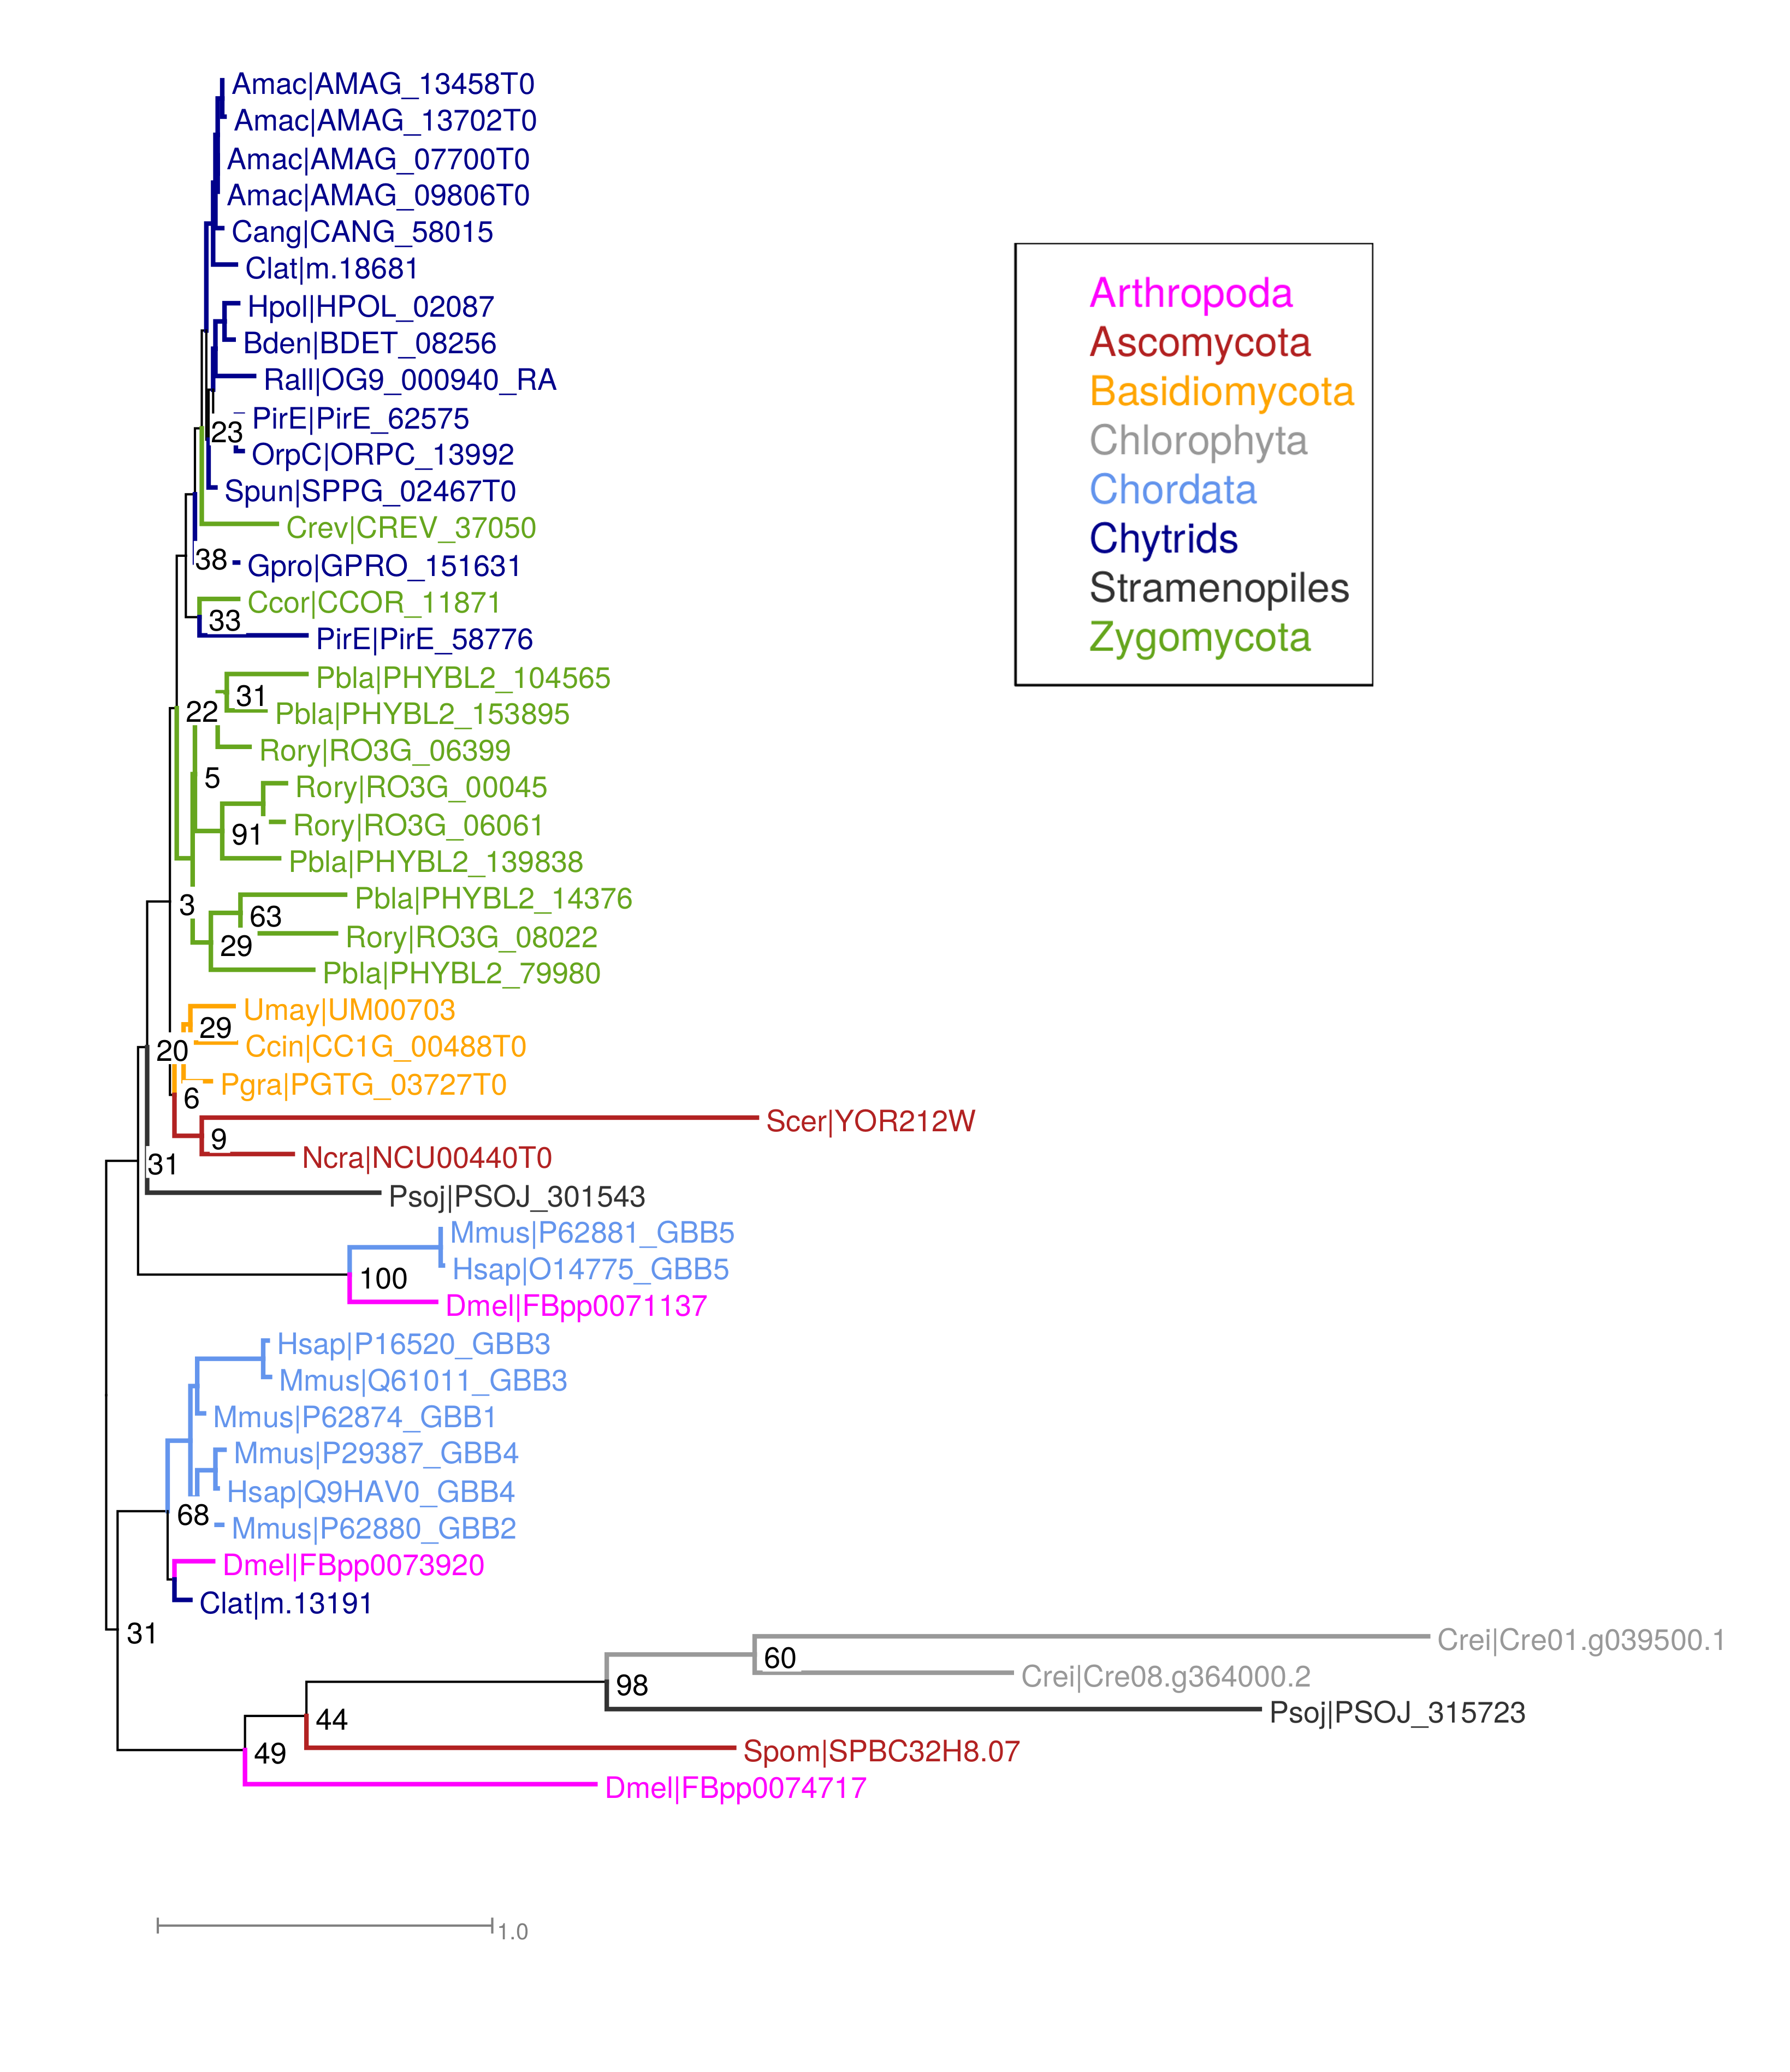
\includegraphics{./Chapter_RhodAux/img/Gbeta_tree.png}
  \caption[Gbeta tree]{Maximum likelihood tree of identified G-beta subunits in fungi and animal outgroups}
  \label{fig:ChRhodA_GbetaTree}
\end{figure}

% Ggamma msa
\begin{figure}[hb]
  \centering
  \begin{texshade}{./Chapter_RhodAux/dat/FungalGG.fasta_aln}
    \threshold[80]{50}
    \setends{1}{45..70}
    \showruler{1}{top}
    \feature{top}{1}{62..65}{brace[Blue]}{Pertussis [Blue]}
    \hidenumbering
  \end{texshade}
  \caption[Galpha MSA]{Multiple sequence aligment of G$\gamma$ proteins identified in fungi which posessed C-terminal pertussis (C[GAVLIP]{2}X) motifs aligned using T-coffee.}
  \label{fig:ChRhodA_ggMSA}
\end{figure}

% Ggamma tree
\begin{figure}[hb]
  \centering
  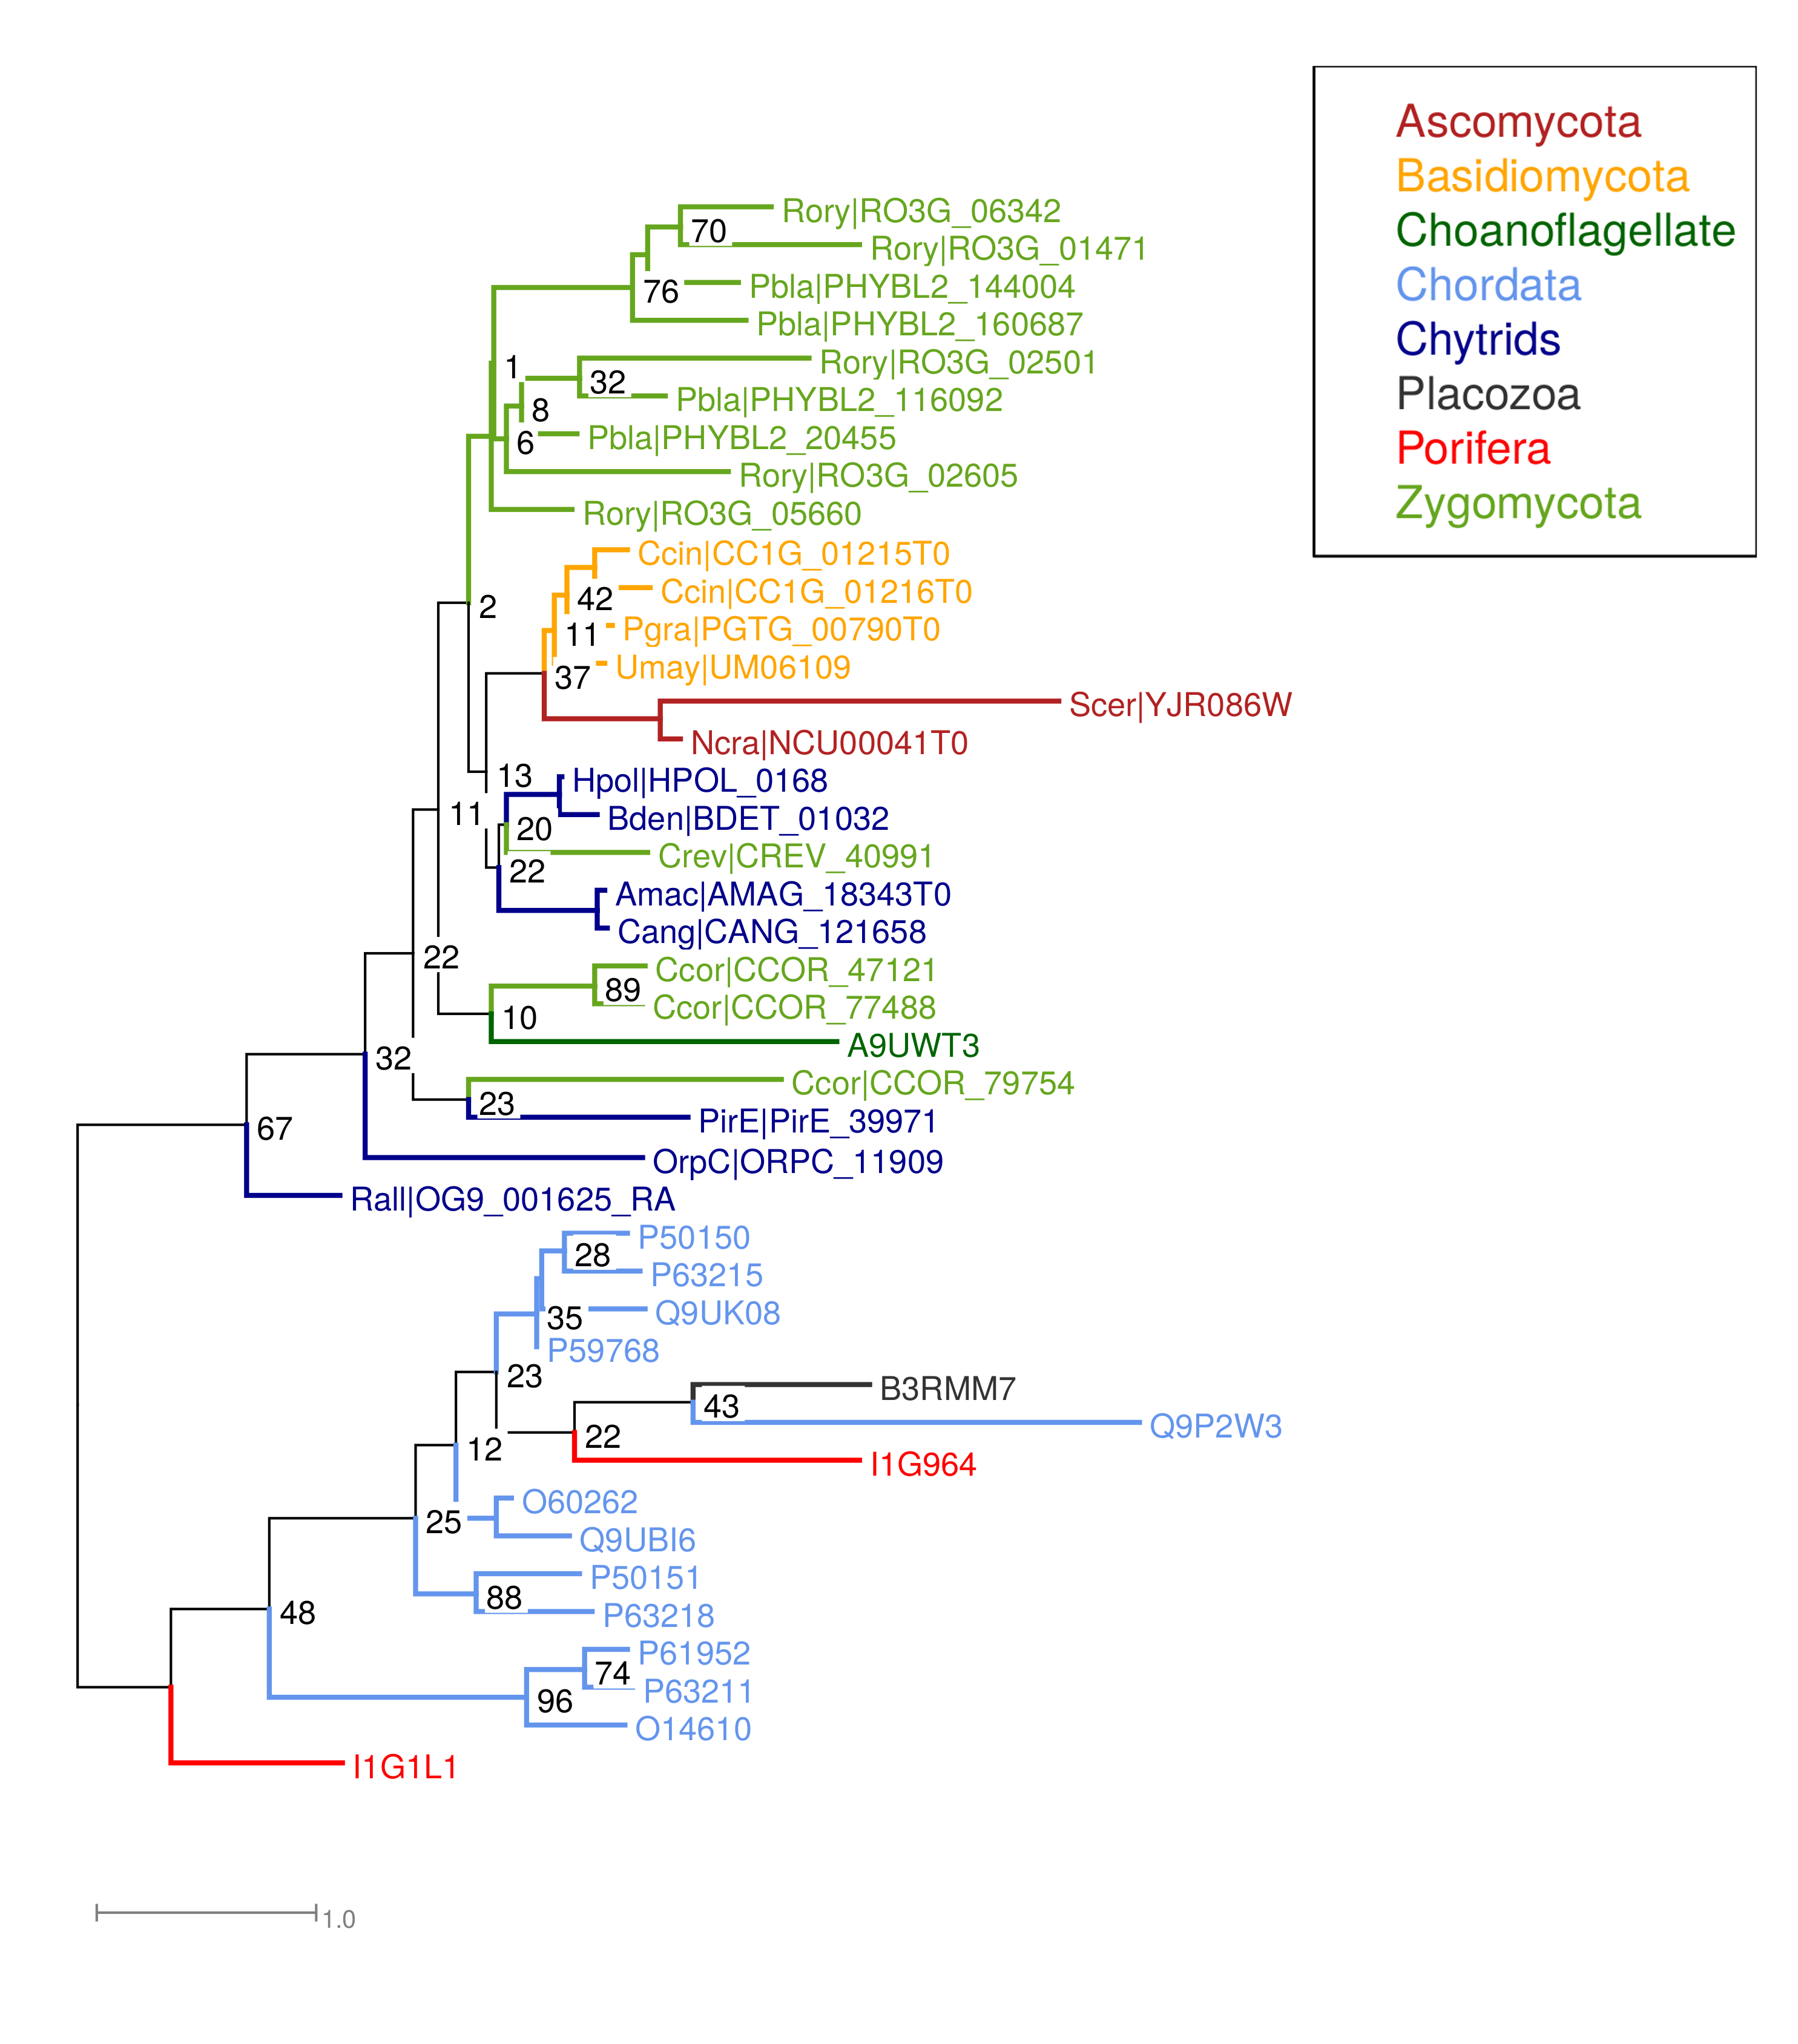
\includegraphics{./Chapter_RhodAux/img/Ggamma_tree.png}
  \caption[Gbeta tree]{Maximum likelihood tree of identified G$\gamma$ subunits in fungi and animal outgroups}
  \label{fig:ChRhodA_GgammaTree}
\end{figure}
